Molekuly na sebe navzájem působí. Důkazů pro to máme více než dost. Pokud by se molekuly na větší vzdálenosti nepřitahovaly, byl by náš svět tvořen jen neposednými molekulami plynů. Naproti tomu pokud by se molekuly na krátkou vzdálenost neodpuzovaly, tak bychom se okamžitě propadli skrze podlahu a nebylo by nám zatěžko procházet zdí. O~povaze odpudivých a~přitažlivých sil začalo být poněkud více jasno od dob Johannese Diderika van der Waalse a jeho studia kondenzace plynů. Často proto nyní mluvíme o~van der waalsovských interakcích jako synonymu slabých mezimolekulových interakcí. Proč se částice přitahují a proč se odpuzují? A~jak silně na sebe částice působí? I~tuto informaci nám poskytne kvantová chemie.

Před tím, než si stručně něco řekneme o~\textit{ab initio} výpočtech slabých mezimolekulových interakcí si provedeme jejich stručnou inventuru. Rozdělíme si je na \uv{klasické} interakce a na interakce \uv{kvantové}.


\subsection{Klasické interakce}
Pod pojmem \uv{klasické} interakce máme na mysli působení vysvětlitelné elektrostatickými silami. Patří sem například

\begin{itemize} 

\item \textbf{Interakce náboj-náboj.} Dva ionty, jeden s~nábojem $q_i$ a druhý s~nábojem $q_j$ na sebe dle Coulombova zákona působí silou

\begin{equation}
E_{int} = \frac{1}{4 \pi \epsilon_0} \frac{q_i q_j}{r_{ij}}.
\label{rov:MS-1}
\end{equation}

\begin{figure} [htb]
\centering
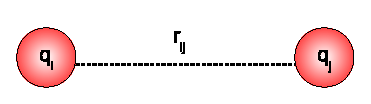
\includegraphics[scale=1]{nabojnaboj.eps}
\caption{Interakce náboj-náboj.}
\label{obr:Naboj-Naboj}
\end{figure}

\item \textbf{Interakce dipól-dipól.} Dvě molekuly s~nenulovým dipólovým momentem na sebe působí interakční energií

\begin{equation}
E_{int} = \frac{-1}{4 \pi \epsilon_0} \frac{\vec{\mu_i} \vec{\mu_j} [ 2 \cos \theta_i \cos \theta_j - \sin \theta_i \theta_j \cos \varphi]}{r_{ij}^3},
\label{rov:MS-2}
\end{equation}

\noindent kde $\vec{\mu}_i$ a $\vec{\mu}_j$ jsou dipólové momenty jednotlivých molekul. Všimněme si, že tato interakce vyhasíná se vzdáleností podstatně rychleji než interakce ion-ion. I~tento vzorec bychom při troše snahy odvodili z~Coulombova zákona. 

\begin{figure} [htb]
\centering
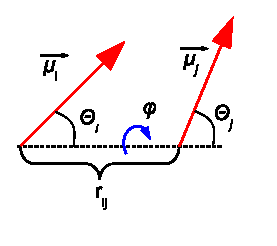
\includegraphics[scale=1]{dipoldipol.eps}
\caption{Interakce dipól-dipól.}
\label{obr:Dipol-Dipol}
\end{figure}

\item \textbf{Interakce dipól-indukovaný dipól.} I~zcela neutrální molekula bez jakýchkoliv elektrických momentů je přitahována k~molekule, která má náboj nebo třeba dipólový moment. V~neutrální molekule se totiž indukuje dipólový moment, který zpětně působí na indukující dipólový moment interakcí typu dipól-dipól. Interakční energie je pak dána jako


\begin{equation}
E_{int} = \frac{-1}{2(4 \pi \epsilon_0)^2} \frac{\vec{\mu_1}^2 \alpha_2 (1 + 3 \cos^2 \theta)}{r^6},
\label{rov:MS-3}
\end{equation}

\begin{figure} [htb]
\centering
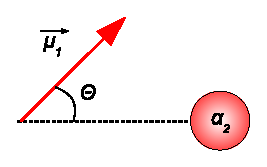
\includegraphics[scale=1]{indukovanydipol.eps}
\caption{Interakce dipól-indukovaný dipól.}
\label{obr:IndukovanyDipol}
\end{figure}

\noindent kde $\alpha_2$ je polarizovatelnost neutrální molekuly a $\mu_1$ je dipólový moment elektricky aktivní molekuly. 

\end{itemize}

Podobným způsobem bychom mohli naleznout vztahy pro interakce ion-dipól, dipól-kvad-rupól či třeba kvadrupól-indukovaný kvadrupól. Všechny tyto interakce lze snadno pochopit na základě fyziky 19. století, kvantové mechaniky zde netřeba. Na druhou stranu ani jedna z~těchto interakcí nevysvětluje, proč kondenzuje do kapalného či pevného stavu kupř. argon, který je prost všech elektrických momentů. Nevíme také pořád, proč nejsme schopni projít zdí.

\subsection{Kvantové interakce}   

Budeme uvažovat dva typy inherentně kvantových interakcí: (Pauliho) repulzi a disperzní interakci.

\begin{itemize} 

\item \textbf{Repulzní interakce.} Dva atomy helia přiblížené na velmi krátkou vzdálenost se začnou odpuzovat. Proč tomu tak je? Na první pohled by se mohlo zdát, že hlavně proto, že se do velké blízkosti dostávají dvě jádra helia, každé z~nich dvojnásobně nabité. To ale není vše, ba není to vůbec to hlavní: na druhou stranu si totiž elektrony vychutnávají přítomnost kladného náboje od druhého atomu. Hlavní problém je v~Pauliho vylučovacím principu. V~každém z~atomů helia se oba elektrony nachází v~1s orbitalu. Pokud se ale snažíme  ze dvou atomů udělat jenom jeden, tak čtyři elektrony se již ve stejném 1s orbitalu nacházet nemohou. Energie tak díky Pauliho repulzi roste. Tato repulze závisí na překryvu mezi příslušnými orbitaly a~můžeme ji proto dobře reprezentovat exponenciální funkcí
   

\begin{equation}
E_{int} = A e^{- \gamma r_{ij}}.
\label{rov:MS-4}
\end{equation}


\item \textbf{Disperzní interakce.} Jde o~přitažlivou interakci, která působí mezi libovolnými dvěma atomy. Někdy se mluví také o~Londonově interakci, dle v~Německu narozeného amerického fyzika Fritze Londona. Jaká je podstata této síly? Díky energii nulového bodu v~kvantové mechanice nikdy neutuchá pohyb. Elektron v~atomu tak neustále kmitá a v~každé chvíli má určitý okamžitý dipólový moment. Tento dipólový moment ale indukuje dipólový moment v~sousedním atomu a oba atomy se tak přitahují interakcí okamžitý dipól-indukovaný dipól. Fritz London odvodil pro tuto interakci přibližný vztah

\begin{equation}
E_{int} \approx \frac{-3}{2 (4 \pi \epsilon_0)^2} \frac{I_A I_B}{I_A + I_B} \frac{\alpha_A \alpha_B}{r_{ij}^6},
\label{rov:MS-5}
\end{equation}

\noindent 
kde $I_A$ a $I_B$ jsou ionizační energie na sebe působících molekul A~a B a~analogicky $\alpha_A$ a~$\alpha_B$ jsou polarizovatelnosti těchto molekul.  
\end{itemize}

\subsection{\textit{Ab initio} výpočty slabých mezimolekulových interakcí}

V~minulých oddílech jsme si představily celou řadu vztahů, které popisují jednotlivé typy slabých mezimolekulových interakcí. Na první pohled tak vše vypadá růžově. Stačí nám vypočítat si metodami kvantové chemie vlastnosti jednotlivých molekul, tedy jejich náboj, dipólový případně vyšší momenty, polarizovatelnost či ionizační energii a poté s~použitím vztahů \eqref{rov:MS-1} až \eqref{rov:MS-5} snadno dopočítáme, jak na sebe molekuly působí. Bohužel pro složitější molekuly takto postupovat nelze a je třeba interakční energii pro vzájemné působení molekul vypočítat přímo. Popíšeme si nyní dvě možné strategie takovéhoto výpočtu.


\subsubsection{Poruchový výpočet: Symetricky adaptovaná poruchová teorie}

Slabé mezimolekulové interakce v~sobě obsahují ono návodné adjektivum \uv{slabé}. Interakce mezi dvěma molekulami tedy může být nahlížena jako malá porucha při pohybu elektronů v~jednotlivých atomech. Podívejme se na jednoduchý případ dvou atomů helia v~určité vzdálenosti.


\begin{figure} [htb]
\centering
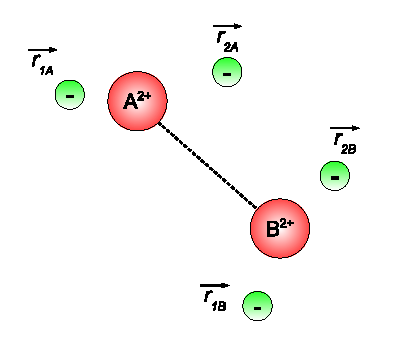
\includegraphics[scale=1]{atomhelia.eps}
\caption{Geometrie atomu helia.}
\label{obr:AtomHelia}
\end{figure}


Elektronový hamiltonián můžeme v~atomových jednotkách zapsat jako


\begin{eqnarray}
\hat{H}_{el} &=&  \underbrace{- \frac{1}{2} (\Delta_{1A} + \Delta_{2A}) + \left( \frac{1}{\vert \vec{r}_{1A} - \vec{r}_{2A} \vert} - \frac{2}{\vert \vec{r}_{1A} - \vec{R_A}\vert} - \frac{2}{\vert \vec{r}_{2A} - \vec{R_A} \vert} \right)}_{\hat{H}_A} \nonumber \\
&-& \underbrace{\frac{1}{2} (\Delta_{1B} + \Delta_{2B}) + \left( \frac{1}{\vert \vec{r}_{1B} - \vec{r}_{2B} \vert} - \frac{2}{\vert \vec{r}_{1B} - \vec{R_B}\vert} - \frac{2}{\vert \vec{r}_{2B} - \vec{R_B} \vert} \right)}_{\hat{H}_B} \nonumber \\
&+&  \bigg( \frac{4}{\vert \vec{R_A} - \vec{R_B}\vert} + \frac{1}{\vert \vec{r}_{1A} - \vec{r}_{1B} \vert} + \frac{1}{\vert \vec{r}_{1A} - \vec{r}_{2B}\vert} + \frac{1}{\vert \vec{r}_{2A} - \vec{r}_{1B} \vert} + \frac{1}{\vert \vec{r}_{2A} - \vec{r}_{2B} \vert} \nonumber \\
&-&  \frac{2}{\vert \vec{r}_{1A} - \vec{R_B} \vert} - \frac{2}{\vert \vec{r}_{2A} - \vec{R_B} \vert} - \frac{2}{\vert \vec{r}_{1B} - \vec{R_A} \vert} - \frac{2}{\vert \vec{r}_{2B} - \vec{R_A} \vert} \bigg),
\label{rov:MS-6}
\end{eqnarray}

\noindent což lze rozepsat jako 

\begin{equation}
\hat{H}_{el} = \underbrace{\hat{H}_A + \hat{H}_B}_{\hat{H}_A^{(0)}} + \hat{H}_{AB}.
\label{rov:MS-7}
\end{equation}

\noindent Řešení rovnice 

\begin{equation}
\hat{H}_{A}^{(0)} \psi_{el}^{(0)} = E_{el}^{(0)} \psi_{el}^{(0)},
\label{rov:MS-8}
\end{equation}

\noindent kde 

\begin{equation}
\hat{H}_A^{(0)} = \hat{H}_A + \hat{H}_B
\label{rov:MS-9}
\end{equation}


\noindent snadno získáme metodou separace proměnných

\begin{equation}
\psi_{el}^{(0)} = \psi_A (\vec{r}_{1A}, \vec{r}_{2A}) \psi_B (\vec{r}_{1B},\vec{r}_{2B}),
\label{rov:MS-10}
\end{equation}


\noindent kde $\psi_A$ je vlnová funkce prvního atomu helia a $\psi_B$ je vlnová funkce druhého atomu helia. Interakční energii pak můžeme vypočítat v~rámci poruchové teorie jako


\begin{equation}
E^{(1)} = \int \psi_{el}^{(0)} \hat{H}_{AB} \psi_{el}^{(0)} \mathrm{d} \vec{r}_{1A} \mathrm{d} \vec{r}_{2A} \mathrm{d} \vec{r}_{1B} \mathrm{d} \vec{r}_{2B}.
\label{rov:MS-11}
\end{equation}


Vypadá to vše jednoduše, ale bohužel je tam zádrhel. Vlnová funkce \eqref{rov:MS-10} není antisymetrická vůči záměně elektronů mezi oběma atomy helia. Je třeba celý postup upravit, mluvíme pak o~symetricky adaptované poruchové teorii (SAPT, z~angl. \textit{Symmetry Adapted Perturbation Theory}). 


\subsubsection{Supramolekulární přístup}
V~rámci supramolekulárního výpočtu vyjádříme interakční energii jako rozdíl energie molekulárního komplexu $E_{AB}$ a energií jednotlivých komponent $E_A$ a $E_B$

\begin{equation}
E_{int} = E_{AB} - E_A - E_B.
\label{rov:MS-12}
\end{equation}


Přístup je to velmi přímočarý a zdá se, že nemůže zklamat. Má ale své problémy. Energie molekul nikdy nepočítáme přesně, ale vždy v~rámci nějaké přibližné metody. I~ty nejnáročnější přístupy poskytují pro realistické systémy hodnoty energií, které se v~absolutní hodnotě od skutečné hodnoty značně liší. Naštěstí větší část chyby se při výpočtu komplexu a komponent vzájemně vyruší, v~chemii nám totiž většinou jde pouze o~rozdíly energií. V~případě slabých mezimolekulových sil nicméně počítáme velmi malou energii jako rozdíl velikých (a skoro stejných) čísel, \uv{snažíme se zjistit hmotnost kapitána jako rozdíl hmotnosti kapitána s~parníkem a~samotného parníku}. V~takovém případě se začnou uplatňovat i jinak zanedbatelné efekty.

Jedním z~problémů je tzv. superpoziční chyba. Jde o~následující problém. Pokud provádíme variační výpočet, tak  víme, že čím větší báze, tím nižší energie. Jestliže nyní provádíme výpočet molekulového komplexu A...B, tak molekula A~v~komplexu může při výpočtu využít i bázových funkcí poskytnutých molekulou B. Dojde ke snížení energie, které není dáno fyzikální interakcí, ale jde toliko o~matematický artefakt. Komplex se pak jeví stabilnější než ve skutečnosti je. Tento defekt odstraňujeme tzv. \textit{counterpoise} korekcí. Interakční energii komplexu vyjádříme jako 

\begin{equation}
E_{int} = E_{AB} - E_{A,[B]} - E_{B,[A]},
\label{rov:MS-13}
\end{equation}

\noindent kde $E_{A,{[B]}}$ je energie atomu A~vypočítaná za přítomnosti báze atomu B a $E_{B,{[A]}}$ je energie atomu B vypočítaná za přítomnosti báze atomu A. Vyvážíme tak neférovou výhodu, které se dostalo atomům A a B v~komplexu A...B.
